%\documentclass[a4paper,english,12pt,twocolumn]{article}
\documentclass[a4paper,english,12pt]{article}
\usepackage[utf8]{inputenc} % Encodage du fichier
\usepackage[T1]{fontenc} % Encodage des fonts nécessaire pour le Latin
\usepackage[french]{babel} % Pour changer la langue des mots générés et choisir la bonne mise en page
\usepackage{amssymb}
\usepackage{pdflscape}
\usepackage{microtype} 
\usepackage{lmodern} % Le latin modèrne
\usepackage[top=2cm, bottom=2cm, left=2.5cm, right=1.5cm]{geometry} % Définir les marges de la page 
\usepackage[hidelinks,urlcolor=blue,unicode=true,
pdftitle={Twitter sentiment analysis},
pdfauthor={BELOUADAH Eden and BOUHAHA Mariem},
pdfdisplaydoctitle=true]{hyperref} % Pour les liens 
\usepackage{fancyhdr} % Pour le style de la page
\usepackage[font=it]{caption} % Rendre les titres des tableaux italiques
\usepackage{graphicx} % Pour les images
\usepackage{subcaption} % Pour mettre plusieurs images sur la même ligne
\usepackage{float} % Pour empêcher le déplacement des tableaux et des figures.
\usepackage{babelbib} % Pour changer la langue dans la bibliographie
\usepackage{amsmath} % Pour des fonctions mathématiques
\usepackage{amssymb} % Pour les symboles mathématiques
%\usepackage[onelanguage,english,longend,boxruled,algoruled,linesnumbered,algochapter,nofillcomment]{algorithm2e} %pour les algorithmes
\usepackage{multirow}
\usepackage{booktabs}
\usepackage{enumitem}
\usepackage{setspace}
\usepackage{longtable}
\graphicspath{ {images/} } 

\DisableLigatures[f]{encoding=*}

%Active ça si tu ne veux pas les points-virgules dans les algorithmes
% \DontPrintSemicolon
 
%\renewcommand \thechapter{\Roman{chapter}} % Utiliser les numéros romans pour les chapitres

\captionsetup{labelfont=it,textfont=it,labelsep=period} % Changer le style des légendes
\AtBeginDocument{ % Changer les légendes
	\renewcommand\tablename{\itshape Tableau}
	\renewcommand{\figurename}{\itshape Figure}
	% Renommer la table des matières
	\renewcommand{\contentsname}{Sommaire}
}

% Style de l'entête et le pied de la page
\setlength{\headheight}{16pt}
\pagestyle{fancy}
\fancyhead[L]{} % Enlever la section
\fancyhead[R]{\footnotesize\slshape{\nouppercase{\leftmark}}} % Titre du chapitre en minuscule avec taille 10
\fancyfoot[C]{}
\fancyfoot[R]{\thepage} % Déplacer le numéro de la page vers la droite de la page

\fancypagestyle{plain}{
\renewcommand{\headrulewidth}{0pt}
\fancyhf{}
\fancyfoot[R]{\thepage}
}
  
% Espace entre les lignes
\linespread{1.3}

% Code pris de https://tex.stackexchange.com/a/95616/109916 et corrigé
% Début
\makeatletter
\newcommand{\emptypage}[1]{
  \cleardoublepage
  \begingroup
  \let\ps@plain\ps@empty
  \pagestyle{empty}
  #1
  \cleardoublepage
  \endgroup}
\makeatletter
% Fin


% pour changer les deux points des légendes d'algorithmes
% \SetAlgoCaptionSeparator{\unskip.}

\begin{document}
%\include{Page_de_garde}
%\include{Remerciements}
\emptypage{
%\tableofcontents
%\listoffigures
%\listoftables
}
    
\setlength{\parskip}{0.6em plus 0.1em minus 0.1em}
%\SetKwInput{KwOut}{Outpits}

% Redéfinition des chapitres et sections pour les inclure dans le sommaire
\makeatletter
%	\let\oldchapter\chapter
%	\newcommand{\@chapterstar}[1]{\cleardoublepage\phantomsection\addcontentsline{toc}{chapter}{#1}{\oldchapter*{#1}}\markboth{#1}{}}
%	\newcommand{\@chapternostar}[1]{{\oldchapter{#1}}}
%	\renewcommand{\chapter}{\@ifstar{\@chapterstar}{\@chapternostar}}
\let\oldsection\section
\newcommand{\@sectionstar}[1]{\phantomsection\addcontentsline{toc}{section}{#1}{\oldsection*{#1}}}
\newcommand{\@sectionnostar}[1]{{\oldsection{#1}}}
\renewcommand\section{\@ifstar{\@sectionstar}{\@sectionnostar}}	
\newcommand*{\rom}[1]{\expandafter\@slowromancap\romannumeral #1@}
\makeatother

\setcounter{page}{1}
%%%%%%%%%%%%%%%%%%%%%%%%%%%%%%%%%%%%%%%%%%%%%%%%%%%%%%%%%%%%%

\title{Twitter Sentiment Analysis: A comparative approach}

\author{Mariem BOUHAHA \and Eden BELOUADAH}
% \date{}
\maketitle



\section{Introduction}
Text classification is a class of problems that finds application in many tasks, mainly sentiment analysis, predicting movie reviews as well as classifying emails as spam or not.

In recent literature, deep learning seems to be promising for text classification, achieving state-of-the-art results on a suite of standard  benchmark problems. 

In this project, we aim to compare and analyze the performance of several deep architectures that we use for sentiment analysis from tweets. For that, we studied the behavior of some deep neural networks as well as the influence of data representation on the models' performances. 

In this intermediate report, we will present the data in hand as well as some statistics to describe it, then we will give a brief description of the models tested so far and finally present the preliminary results. 

\section{Presenting the data}
For this project, we used the B-task SemEval-2013 training and development data, which have the following characteristics before any preprocessing:

\begin{table}[H]\centering
\begin{tabular}{|c|c|c|c|c|}

\hline
Set & Number of examples & Positive & Negative & Neutral\\
\hline
Train & 5916 & 2179 & 816 & 2921\\
\hline
Development & 876 & 324 & 158 & 394\\
\hline

\end{tabular}
\caption{Classes distribution for trainset and devset}
\end{table}

If we visualize an extract (the first 5 for example) of the tweets in the training set, we get the text shown in figure \ref{extract}.

\begin{figure}[h!]
\centering
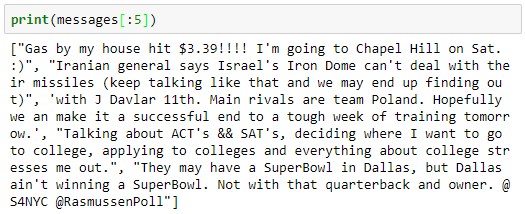
\includegraphics[scale=1]{extract}
\caption{A small extract from Train}
\label{extract}
\end{figure}

We noticed that, in addition to words, messages contain hashtags, URLs and user tags, which are less likely to be useful for sentiment prediction. 

We also computed some statistics for the tweets, which we summarize in table \ref{stat}.


\begin{table}[H]\centering
	\begin{tabular}{|c|c c c|c c c|c c c|}
		\hline \textbf{Type}  & \multicolumn{3}{|c|}{\textbf{Positive messages}} & \multicolumn{3}{|c|}{\textbf{Negative messages}} & \multicolumn{3}{|c|}{\textbf{Neutral messages}}\\    \hline
		 Length & Min & Max & Mean & Min & Max & Mean & Min & Max & Mean\\   \hline
		\textbf{Train} & 4&44&23&6&38&23&5&40&23 \\
		\textbf{Dev} & 7&35&23&8&34&23&6&38&22 \\
		\hline
	\end{tabular}
	\caption{Statstics about messages length for trainset and devset before data preprocessing}
	\label{stat}
\end{table}


\section{Data Preprocessing}
Since we cannot use the "dirty" raw text tweets for classification, we did some preprocessing as following:
\begin{itemize}
	\item Tokening messages using \emph{NLTK Tweet Tokenizer} which is more appropriate for this type of messages,
	\item Using regular expressions to remove digits (24, 12.400\$...), punctuations (?,:,;,",\#, @...), tags (@user) and every sequence of special characters. Howerver, the emoticons are kept,
	\item Using $NLTK Stop words$ to remove all useless words,
	\item Preprocessing Hashtags: removing \# and separating the hashtag parts (\#VeryHappy -> Very + Happy)
	\item Transform all messages to lower case. 
\end{itemize}

These operations left us with a training vocabulary of size 17284, where preprocessed tweets now have the following statistics:


\begin{table}[H]\centering
	\begin{tabular}{|c|c c c|c c c|c c c|}
		\hline \textbf{Type}  & \multicolumn{3}{|c|}{\textbf{Positive messages}} & \multicolumn{3}{|c|}{\textbf{Negative messages}} & \multicolumn{3}{|c|}{\textbf{Neutral messages}}\\    \hline
		Length & Min & Max & Mean & Min & Max & Mean & Min & Max & Mean\\   \hline
		\textbf{Train} & 3&22&12&3&20&13&3&22&12 \\
		\hline
	\end{tabular}
	\caption{Statstics about messages length for trainset and devset after data preprocessing}
\end{table}


As we notice, tweets have different lengths. To handle this, we take the size of the longest message and use it as a reference. The tweets having the same number of words are kept as they are, and shorter ones are replicated until their size become equal to that of the longest tweet.


In figure \ref{freq}, we show the distribution of word frequencies in our training set. 

\begin{figure}[h!]
\centering
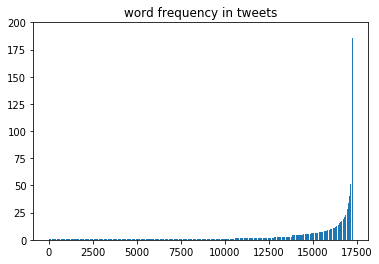
\includegraphics[scale=1]{freq}
\caption{Word frequency}
\label{freq}
\end{figure}

\section{Models and results}
\subsection{Long Short Term Memory (LSTM)}
The first reflex that we had when handling text data is to use recurrent neural networks. LSTM is one of the most used types of language models.

In this first work, we are using batch mode with the following architecture:
\begin{itemize}
	\item Number of layers: 1,
	\item Number of hidden units: 150,
	\item Knowing that we have three classes in our classification problem, the LSTM layer is connected to a linear layer of size (number of hidden units X3).
	\item Optimizer: We used Adam optimizer instead of smple SGD since the latter is less robust against local optima.
	\item Loss: We used the Cross Entropy Loss. 
\end{itemize}

After peforming forward propagation, we backward the error and update the parameters of the model.

The program shows real time plots for accuracy and the Cross Entropy Loss.

\begin{figure}[H]
\centering
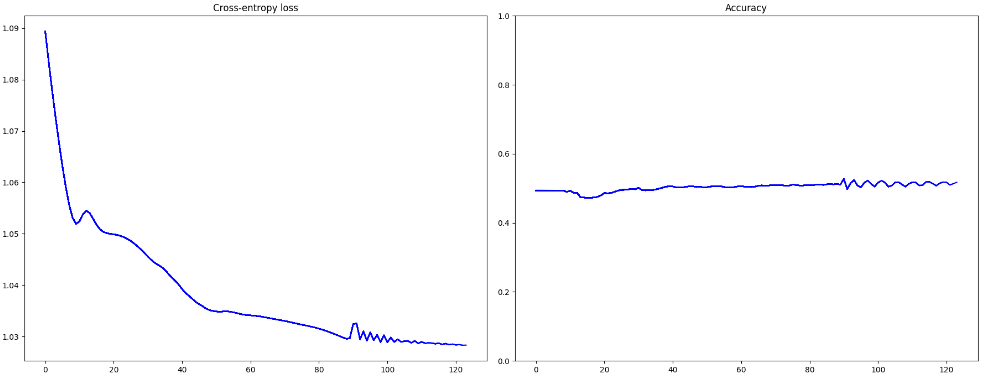
\includegraphics[scale=0.85]{acc_loss}
\caption{Accuracy and Loss evolution for LSTM baseline}
\end{figure}

Unfortunately, The maximum of accuracy that our model reached is 52\%. We think about changing again the architecture of the model, probably change the data preprocessing and why not add dropout techniques.

\subsection{Multi-Layer Perceptron (MLP)}


\section{Conclusion}
In this intermediate report we showed data preprocessing and our baseline results. We are aiming to make the models give a higher accuracy and a lower prediction error. We hope that the final report will be more convincing.  

\end{document}
